\documentclass[10pt, a4paper]{article}
\usepackage{lingmacros}
\usepackage{diagbox}
\usepackage{tree-dvips}
\usepackage[T1]{fontenc}
\usepackage[polish]{babel}
\usepackage[utf8]{inputenc}
\usepackage{csquotes}
\usepackage{multirow}
\usepackage{biblatex}
\usepackage{graphicx}
\usepackage{float}
\usepackage{caption}
\usepackage{hyperref}
\usepackage{cleveref}
\usepackage{pgfplots,wrapfig}
\bibliography{bibliography}
\begin{document}
    \author{Juliusz Straszyński}
    \title{Raport końcowy projektu}
    \maketitle
    \tableofcontents


    \section{Wstęp}\label{sec:wstep}
    28 stycznia 2006 roku całą Polską wstrząsnęła tragedia — pod naporem śniegu zawaliła się hala MTK, w wyniku czego
zginęło 65 osób.
Po tym wydarzeniu firma WISENE Roof Monitoring opracowała rozwiązanie, które może zapobiec tego
typu katastrofom.
Projekt opiera się na zainstalowaniu szeregu precyzyjnych czujników laserowych, z których pomiaru można wywnioskować stopień ugięcia dachu.
Czujniki mogą być ustawione poziomo pod dachem, pod kątem, lub pionowo, precyzyjnie wykrywając milimetrowe ugięcia dachu.

Siłą przedstawionego rozwiązania jest jego prostota — nie potrzeba skomplikowanego przygotowania, by zainstalować taki system.
Laserowe czujniki są tanie w utrzymaniu, zarówno materiałowo, jak i organizacyjnie.
Natomiast wadą systemu jest jego wrażliwość na możliwe zaburzenia pomiarów odległości.
Przy zainstalowaniu takiego systemu w działających przedsiębiorstwach, nieuniknione jest potencjalne zastawienie czujników.
Zastawienia mogą być bardzo wyraźne — np.\ po ustawieniu dwumetrowej szafy, ale też mogą być delikatne — w wyniku dłuższego pozostawienia paczki papierosów.
%\begin{wrapfigure}{r}{0.25\textwidth}
%    \centering
%    \begin{tikzpicture}[]
%        \path[draw]
%  (0.0, 0.0)
%        -- (0.0, 1.0)
%        (1.0, 1.0)
%        -- (1.0, 0.0)
%        (1.0, 0.0)
%        -- (0.0, 0.0);
%        \path[draw, bend left]	(0.0, 1.0)	to[in=-150, out=-30] (1.0, 1.0);
%    \end{tikzpicture}
%    \caption{Wraz z obciążeniem dachu, maleje odległość czujnika od zadaszenia do podłoża.}
%\end{wrapfigure}

Celem tego projektu jest zażegnanie tego problemu poprzez opracowanie ulepszonego systemu raportującego, czy pomiar czujnika jest zastawiony, czy nie.
Jest to kluczowy komponent systemu, ponieważ jego brak może powodować zbyt częste raportowanie fikcyjnych ugięć, a co za tym idzie, ignorowania raportowanych alarmów.
Ponadto system szacuje prawdopodobną wartość wykrytego zastawienia.


    \section{Analiza danych}\label{sec:analiza-danych}
    \subsection{Struktura}\label{subsec:struktura}
W sumie przeanalizowanych zostało 135 zestawów danych.
Pojedynczy zestaw danych składa się z pomiarów czujników rozmieszczonych w różnych miejscach na pojedynczym obiekcie.
Liczba czujników waha się od kilku do kilkudziesięciu.
Każdy czujnik jest scharakteryzowany przez następujące dane:
\begin{itemize}
    \item identyfikator,
    \item odległość bazowa — oznaczająca odległość zmierzoną przez laserowe urządzenie pomiarowe, w chwili uruchomienia monitoringu na obiekcie,
    \item seria pomiarów — notująca odległość czujnika od podłoża w kolejnych momentach.
\end{itemize}
Rozwiązanie zostało opracowane na podstawie pomiarów 1225 urządzeń i około 600 tys.\ pomiarów odległości.

\subsection{Charakterystyka}\label{subsec:charakterystyka}

\subsubsection{Odstępy czasu}
\begin{figure}[h]
    \centering
    % This file was created with tikzplotlib v0.9.12.
\begin{tikzpicture}

\definecolor{color0}{rgb}{0.886274509803922,0.290196078431373,0.2}

\begin{axis}[
axis background/.style={fill=white!89.8039215686275!black},
axis line style={white},
log basis y={10},
tick align=outside,
tick pos=left,
x grid style={white},
xlabel={Odstępy czasu między kolejnymi pomiarami [minuty]},
xmajorgrids,
xmin=98.5, xmax=1341.5,
xtick style={color=white!33.3333333333333!black},
y grid style={white},
ylabel={liczba wystąpień},
ymajorgrids,
ymin=119.838906477549, ymax=6012830.80078,
ymode=log,
ytick style={color=white!33.3333333333333!black}
]
\draw[draw=black,fill=color0,line width=0.48pt] (axis cs:335,0) rectangle (axis cs:385,1873303);
\draw[draw=black,fill=color0,line width=0.48pt] (axis cs:155,0) rectangle (axis cs:205,3676383);
\draw[draw=black,fill=color0,line width=0.48pt] (axis cs:695,0) rectangle (axis cs:745,1595);
\draw[draw=black,fill=color0,line width=0.48pt] (axis cs:515,0) rectangle (axis cs:565,611);
\draw[draw=black,fill=color0,line width=0.48pt] (axis cs:1055,0) rectangle (axis cs:1105,479);
\draw[draw=black,fill=color0,line width=0.48pt] (axis cs:1235,0) rectangle (axis cs:1285,196);
\draw[draw=black,fill=color0,line width=0.48pt] (axis cs:875,0) rectangle (axis cs:925,235);
\end{axis}

\end{tikzpicture}

    \captionof{figure}{Zbiorczy histogram przedstawiający odstępy czasu między kolejnymi pomiarami dla wszystkich danych.}\label{fig:odstepyczasu}
\end{figure}

Rysunek~\ref{fig:odstepyczasu} pokazuje, że przez większość czasu okres raportowania wynosi 3 lub 6 godzin.
By ułatwić komputerową analizę, dane zostały przepróbkowane do jednostajnego okresu 3h.
Finalnie, każdy okres jest reprezentowany przez jedną wartość pomiaru.
Każdy przedział czasu z co najmniej jednym pomiarem jest zagregowany do mediany.
Każdy przedział 3-godzinny bez żadnego pomiaru jest reprezentowany przez ostatni pomiar przed tym przedziałem.

Mediana jest tutaj właściwym agregatorem, ponieważ jest ona odporna na duże odchylenia, w przeciwieństwie do np.\ średniej.

\subsubsection{Różnice odległości między kolejnymi pomiarami}

\begin{figure}[h]
    \centering
    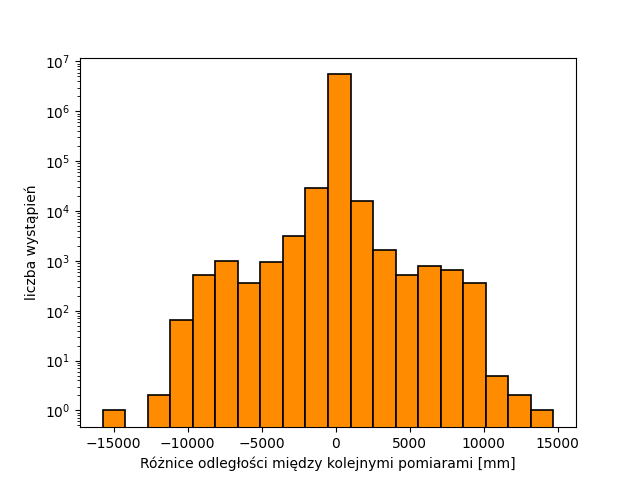
\includegraphics[width=\textwidth]{dist_diff_big.png}\captionof{figure}{Zbiorczy histogram różnic między kolejnymi pomiarami odległości dla wszystkich danych.}
    \label{fig:distbig}
\end{figure}

Bardzo istotne jest to, że na rysunku~\ref{fig:distbig} pionowa skala jest logarytmiczna.
Z informacji dostarczonych przez firmę wiadomo, że bez zastawienia czujnika, różnica pomiaru w ciągu kilku godzin może być co najwyżej 25-milimetrowa.
Ta informacja pokrywa się z wyżej pokazanym wykresem, ponieważ zdecydowana większość obserwacji jest zawarta w tym zakresie.
Bardzo wysoki szpic do 10 milimetrów reprezentuje zdecydowaną większość obserwacji, co widać na rysunku~\ref{fig:diffsmall}.


\begin{figure}[h]
    \centering
    % This file was created with tikzplotlib v0.9.12.
\begin{tikzpicture}

\definecolor{color0}{rgb}{0.886274509803922,0.290196078431373,0.2}

\begin{axis}[
axis background/.style={fill=white!89.8039215686275!black},
axis line style={white},
log basis y={10},
tick align=outside,
tick pos=left,
x grid style={white},
xlabel={Różnice odległości między kolejnymi pomiarami [mm]},
xmajorgrids,
xmin=-26.95, xmax=26.95,
xtick style={color=white!33.3333333333333!black},
y grid style={white},
ylabel={liczba wystąpień},
ymajorgrids,
ymin=226.106279176677, ymax=6677184.14321567,
ymode=log,
ytick style={color=white!33.3333333333333!black}
]
\draw[draw=black,fill=color0,line width=0.48pt] (axis cs:-24.5,0) rectangle (axis cs:-22.05,364);
\draw[draw=black,fill=color0,line width=0.48pt] (axis cs:-22.05,0) rectangle (axis cs:-19.6,646);
\draw[draw=black,fill=color0,line width=0.48pt] (axis cs:-19.6,0) rectangle (axis cs:-17.15,548);
\draw[draw=black,fill=color0,line width=0.48pt] (axis cs:-17.15,0) rectangle (axis cs:-14.7,868);
\draw[draw=black,fill=color0,line width=0.48pt] (axis cs:-14.7,0) rectangle (axis cs:-12.25,803);
\draw[draw=black,fill=color0,line width=0.48pt] (axis cs:-12.25,0) rectangle (axis cs:-9.8,1615);
\draw[draw=black,fill=color0,line width=0.48pt] (axis cs:-9.8,0) rectangle (axis cs:-7.35,1816);
\draw[draw=black,fill=color0,line width=0.48pt] (axis cs:-7.35,0) rectangle (axis cs:-4.9,6412);
\draw[draw=black,fill=color0,line width=0.48pt] (axis cs:-4.9,0) rectangle (axis cs:-2.45,25374);
\draw[draw=black,fill=color0,line width=0.48pt] (axis cs:-2.45,0) rectangle (axis cs:0,1174980);
\draw[draw=black,fill=color0,line width=0.48pt] (axis cs:0,0) rectangle (axis cs:2.45,4182142);
\draw[draw=black,fill=color0,line width=0.48pt] (axis cs:2.45,0) rectangle (axis cs:4.9,20956);
\draw[draw=black,fill=color0,line width=0.48pt] (axis cs:4.9,0) rectangle (axis cs:7.35,5312);
\draw[draw=black,fill=color0,line width=0.48pt] (axis cs:7.35,0) rectangle (axis cs:9.8,1646);
\draw[draw=black,fill=color0,line width=0.48pt] (axis cs:9.8,0) rectangle (axis cs:12.25,1517);
\draw[draw=black,fill=color0,line width=0.48pt] (axis cs:12.25,0) rectangle (axis cs:14.7,760);
\draw[draw=black,fill=color0,line width=0.48pt] (axis cs:14.7,0) rectangle (axis cs:17.15,824);
\draw[draw=black,fill=color0,line width=0.48pt] (axis cs:17.15,0) rectangle (axis cs:19.6,468);
\draw[draw=black,fill=color0,line width=0.48pt] (axis cs:19.6,0) rectangle (axis cs:22.05,577);
\draw[draw=black,fill=color0,line width=0.48pt] (axis cs:22.05,0) rectangle (axis cs:24.5,361);
\end{axis}

\end{tikzpicture}

    \captionof{figure}{Zbiorczy histogram różnic między kolejnymi pomiarów odległości dla wszystkich danych. Obcięty do 25mm.}
    \label{fig:diffsmall}
\end{figure}

\subsubsection{Różnice bazy od odległości}
\begin{figure}[h]
    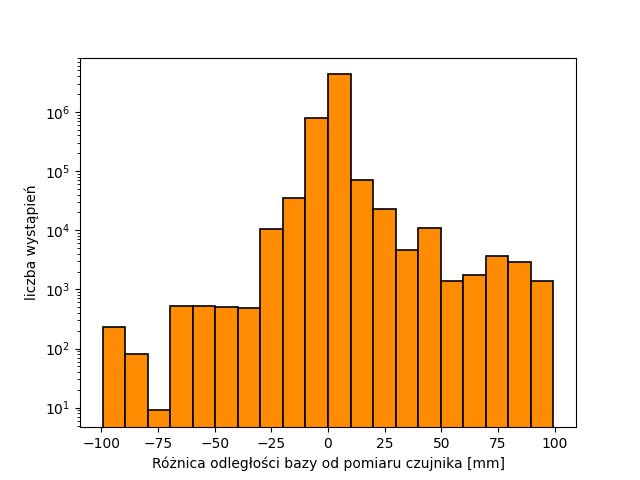
\includegraphics[width=\textwidth]{dist_histogram_100.png}
    \captionof{figure}{Zbiorczy histogram różnic odległości bazowej od pomiarów odległości.}
    \label{fig:dist}
\end{figure}


Dane na rysunku~\ref{fig:dist} są ponownie przedstawione w skali logarytmicznej, bo w przeciwnym wypadku nie dałoby się niczego zauważyć.
Zdecydowana większość obserwacji oscyluje wokół zera.
Mediana jest równa zero.
Będzie to kluczowe — prawdziwe ugięcia dachu powinny być krótkotrwałe i w dłuższej perspektywie mediana pomiarów powinna wynosić zero.

\subsubsection{Autokorelacja}\label{subsubsec:autocorrelation}

Na rysunku~\ref{fig:autocorrelation} pokazana jest zbiorcza autokorelacja wszystkich szeregów czasowych pomiarów z każdego czujnika, indeksowana przesunięciem (ang.\ lag).
Niebieskim cieniem jest zaznaczony przedział ufności (ang.\ \emph{confidence interval}), który pokazuje które korelacje są statystycznie istotne.

Zatem autokorelacja jest na tyle statystycznie istotna, że można zamodelować szereg czasowy pomiarów czujników autoregresją z oknem o długości 20.
\begin{figure}[H]
    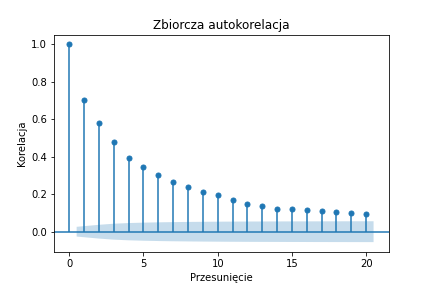
\includegraphics[width=0.9\textwidth]{autocorrelation.png}
    \captionof{figure}{Zbiorcza autokorelacja różnicy odległości bazowej od pomiaru dla wszystkich zestawów danych.}
    \label{fig:autocorrelation}
\end{figure}

\subsubsection{Omówienie wybranych przykładów}

Dane z urządzenia \hyperref[fig:example812]{JTI OTP - Gostków Stary/P-3}, pokazują przykład zastawienia 13mm trwającego przez wrzesień roku 2020.
Natomiast ostatnia część wykresu pokazuje faktyczne ugięcie dachu spowodowane śniegiem w lutym 2021.
Wspomniane warunki pogodowe wyróżniają się np.\ również w danych z urządzenia \hyperref[fig:example201]{C-Lublin - Lublin /P4}.





    \section{Metodologia i algorytm}\label{sec:metodologia-i-algorytm}
    \section{Metodologia i algorytm}
\subsection{Wstęp}
Każdy zestaw danych składa się z kilku szeregów czasowych. W tych szeregach czasowych mamy zidentyfikować anomalie (ang.\ \emph{outlier}, \emph{anomaly}). Jest to znany problem w analizie statystycznej, do którego mamy do dyspozycji opracowane wcześniej narzędzia. Dziedziną zajmującą się rozpoznawaniem anomalii jest \emph{intervention analysis}.

Prawdopodobnie najważniejszą pracą w tej dziedzinie jest praca Ruey S. Tsaya \citetitle{https://doi.org/10.1002/for.3980070102} \cite{https://doi.org/10.1002/for.3980070102}. Jest ona powszechnie cytowanym fundamentem współczesnej analizy anomalii w szeregach czasowych.

Najistotniejsze jest zidentyfikować, czym tak naprawdę jest zastawienie z punktu widzenia intervention analysis. Zastawienie tymczasowo zmienia bazę pomiarów miernika. Oznacza to, że na czas zastawienia, pomiary są zmienione o pewną wysokość. Używając terminologii z ww. pracy jest to klasyfikowane jako \emph{level shift}. Jeśli zastawienie jest krótkotrwałe, to bardziej pasuje termin \emph{spike}.

Praca Tsaya opiera się głównie na modelach \emph{ARMA}. Model ARMA jest połączeniem dwóch modeli AR i MA, czyli autoregresji i średniej kroczącej. Model (a konkretnie część MA) można stosować pod warunkiem, że analizowany szereg czasowy jest stacjonarny.

Dodatkowo, by nasze rozwiązanie było możliwe do zastosowania w praktyce, musimy raportować wyniki na bieżąco, tj.\ w trybie \textbf{online}. Jest to kluczowe, ponieważ zmniejszy to użyteczność niektórych potencjalnych modeli.
\subsection{Skorelowanie urządzeń}
Jako że na urządzenia z pojedynczego budynku oddziałują praktycznie te same warunki atmosferyczne, to można by, zamiast modelu rozpatrującego każde z urządzeń osobno, spróbować wywnioskować anomalie z braku synchronizacji ruchów między urządzeniami.

Nie zdecydowaliśmy się na to, ze względu na dwa czynniki. Po pierwsze model mógłby się przeuczyć (ang.\ \emph{overfit}) na podstawie tej własności, co sprawiłoby, że fałszywie raportowałby zastawienie w przypadku, gdy tylko część dachu jest obciążona np.\ materiałami budowlanymi, zamiast śniegiem. Po drugie trenowanie modelu na wielowymiarowym szeregu czasowym jest dużo trudniejsze i łatwiej o przeuczenie się. Dlatego właśnie w praktyce, w takich sytuacjach, rozpatruje się szeregi czasowe niezależnie, o ile jest taka możliwość.
\subsection{Metoda rozstępu ćwiartkowego}
Metoda rozstępu ćwiartkowego (ang.\ IQR -- Interquartile range) jest jedną z najprostszych metod rozpoznawania anomalii w szeregu czasowym. Po poszeregowaniu historycznych danych na kwartyle $Q_1, Q_2, Q_3, Q_4$, definiujemy $\mathit{IQR}:= Q_3 - Q_1$, nazywane także \emph{midspread}. Następnie jesteśmy w stanie wykonać prosty Interquartile range test -- sprawdzamy, czy analizowany pomiar jest pomiędzy $Q_1 - c \cdot \mathit{IQR}$ i $Q_3 + c \cdot \mathit{IQR}$, gdzie $c$ to dopuszczalny margines. W naszym przypadku przyjęliśmy $c=3$, by tolerować szeroki zakres obserwacji.
\subsection{Zmiana poziomu}\label[]{levelshift}
Zmiana poziomu (ang.\ \emph{level shift}) jest jednym z głównych typów anomalii analizowanych w pracy \cite{https://doi.org/10.1002/for.3980070102}. By wykrywać takie anomalie, używa się podwójnego przesuwnego okna. Podwójne przesuwne okno jest parametryzowane przez $d$, oznaczające długość skrzydła. Jeśli ostatnie $2d$ pomiarów to $X_1, \ldots X_{2d}$, to lewym skrzydłem jest $X_1, \ldots X_d$, a prawym $X_{d + 1}, \ldots, X_{2d}$. Metryką dla takiego podwójnego przesuwnego okna jest różnica median prawego i lewego skrzydła. Następnie dla tej metryki używamy metody rozstępu ćwiartkowego.

Niestety nie jest to wskaźnik, którego moglibyśmy łatwo użyć w naszym przypadku. Daje on informację z opóźnieniem $d$ obserwacji, ponieważ daje on informację o środkowym elemencie między skrzydłami. Dodatkowo, informacja ta jest zduplikowana -- po niewielkim przesunięciu okna ta metoda nadal notuje anomalię. Przez to ciężko odzyskać faktyczny poziom ugięcia dachu.
\subsection{Nagłe wzrosty}\label{spike}
Nagły wzrost (ang.\ \emph{spike}) jest kolejnym typem anomalii rozpatrywanym w pracy \cite{https://doi.org/10.1002/for.3980070102}. Ten typ anomalii jest wykrywany poprzez przesuwne okno, które jest parametryzowane przez $d$ -- jego rozmiar. Jeśli ostatnie $d + 1$ pomiarów to $X_1, \ldots X_{d + 1}$, to oknem jest $X_1, \ldots X_d$. Metryką jest różnica ostatniego elementu $X_{d+1}$ od mediany okna. Dla takiej metryki używamy metody rozstępu ćwiartkowego. Metoda ta jest wykryje zmianę poziomu w najwcześniejszym momencie, ponieważ początek level shift jest również spikem.
\subsection{Autoregresja}\label{autoregression}
Autoregresja pozwala sprawdzić, czy obserwacje nie odbiegają od poprzedzających w ramach pewnej funkcji liniowej. Jest parametryzowana przez $d$ -- rozmiar okna. Jeśli ostatnie $d + 1$ pomiarów to $X_1, \ldots X_{d + 1}$, to oknem jest $X_1, \ldots X_d$. Dodatkowo, uczymy się parametrów $c_1, \ldots, c_d$. Metryką jest różnica ostatniego elementu $X_{d+1}$ od kombinacji liniowej $c_1X_1 + c_2X_2 + \ldots + c_dX_d$. Parametrów uczymy się za pomocą regresji liniowej na historycznych danych. Dla metryki używamy metody rozstępu ćwiartkowego. Jest to bardzo precyzyjna metoda, która dobrze działa, jeśli mamy wysoki poziom autokorelacji w szeregu czasowym. W naszym przypadku ten warunek jest spełniony.
\subsection{Próg}\label{threshold}
Znając możliwy potencjalny zakres danych, możemy pozbyć się z danych wejściowe najbardziej oczywistych anomalii, które mogłyby zaburzyć bardziej skomplikowane metody jak autoregresja. Każde urządzenie ma maksymalne możliwe ugięcie, po przekroczeniu którego powinien uruchomić się alarm. Możemy ustawić próg na najbardziej oczywiste anomalie na 4-krotność maksymalnego możliwego ugięcia, bo wtedy albo mamy zastawienie, albo dach powinien już się dawno zawalić.
\subsection{Inżynieria danych}
Nasze 135 zestawów danych zostało podzielone na dwie części -- treningową i ewaluacyjną. Treningowa część składa się z danych z 50 losowych urządzeń, natomiast pozostałe zostały wykorzystane do ewaluacji. Dane zostały przepróbkowane do okresu 3 godzin.
\subsection{Rozwiązanie}\label{solution}
Używamy wskaźników z sekcji \ref{spike}, \ref{autoregression} i \ref{threshold}, i obserwacja jest raportowana jako anomalia, jeśli dowolny z tych wskaźników zwróci, że obserwacja jest anomalią.
\subsection{Odrzucone rozwiązania}
Zamiast klasycznej analizy statystycznej, moglibyśmy również spróbować znanych metod uczenia maszynowego, przykładowo sieci neuronowych. Jednakże metody te najczęściej nie radzą sobie z danymi o wysokim poziomie szumu, a z takimi mamy do czynienia w naszym przypadku. Dodatkowo, nie ma problemu z trudnością z interpretowalnością wyników. Zagraniczne korporacje takie jak Facebook nadal używają klasycznych metod statystycznych do wykrywania anomalii \cite{Prophet}, chociaż pojawiają się próby zaadaptowania do współczesnych metod uczenia maszynowego \cite{Neuralprophet}.

Istniejące, bardziej skomplikowane rozwiązania takie jak Prophet Facebooka \cite{Prophet} skupiają się głównie na wahaniach sezonowych (np. weekendy/święta Bożego narodzenia), ponieważ są one przeznaczone dla systemów o dużej skali i nie ma tam konieczności rozpoznania wszystkich anomalii. W naszym przypadku wahania sezonowe mają znaczenie drugorzędne -- mimo że zwykle możemy spodziewać się opadów śniegu w zimie, to nie możemy na tym polegać, gdyż nadmierne obciążenia mogą powstać z innej przyczyny i nadal być niebezpieczne.
\section{Realizacja}
\subsection{Rozwiązanie porównawcze}
Punktem odniesienia będzie bardzo proste rozwiązanie, które stwierdza, że jeśli różnica kolejnych dwóch pomiarów była większa od 25 mm, to było to zastawienie.
\subsection{Implementacja}
Eksploracja danych i trenowanie zostały wykonane w języku programowania Python przy użyciu biblioteki ADTK \cite{ADTK} wydanej w 2019 roku. Następnie, po wytrenowaniu parametrów, program został przepisany na język C++ do postaci prostej biblioteki implementującej wskaźniki wymienione w sekcji \ref{solution}.

Takie rozwiązanie wykrywa zmiany zastawienia. By sprawdzić, czy urządzenie jest w aktualnym momencie zastawione, utrzymujemy licznik zastawienia, który się zmienia wraz z wykrytym zastawieniem.
\subsection{Tabela krzyżowa}
\begin{tabular}{|l||*{2}{c|}}\hline
\backslashbox{Nowy}{Porównawczy}
&\makebox[6em]{Brak}&\makebox[6em]{Zastawienie}\\\hline
Brak &84.0739\%&0.2156\%\\\hline
Zastawienie &9.8976\%&5.8130\%\\\hline
\end{tabular}


Nowy model wykrywa około 3 razy więcej zastawień na danych testowych niż porównawczy model. Modele zgadzają się ok. 90\% przypadków. 98\% z pozostałych 10\% to nowowykryte zastawienia.
\subsection{Przykłady}\label{exampless}
Wykorzystujemy te same przykłady co w \ref{examples}.

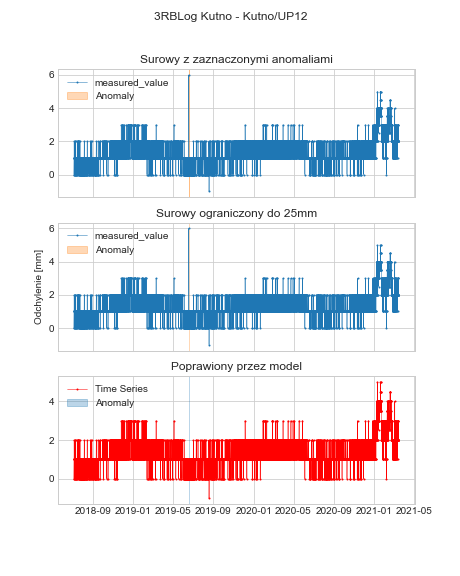
\includegraphics[width=0.9\textwidth]{summary_dev_11.png}

Jedyna anomalia na wysokości 6mm została wykryta i poprawiona.

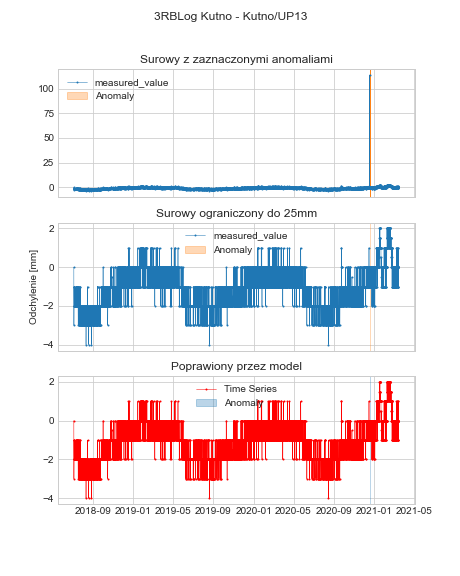
\includegraphics[width=0.9\textwidth]{summary_dev_12.png}

Anomalia na wysokości 120mm została wykryta i poprawiona.

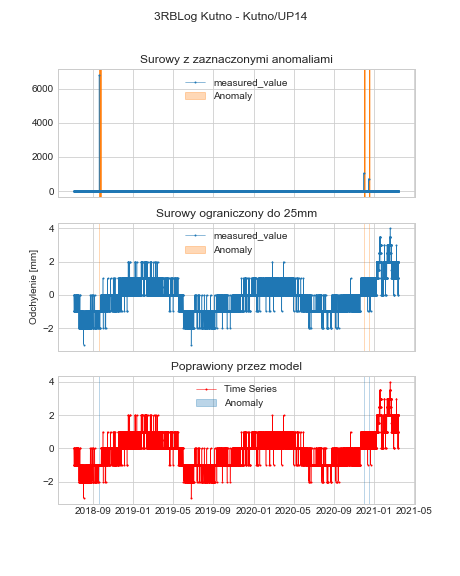
\includegraphics[width=0.9\textwidth]{summary_dev_13.png}

Anomalie na wysokości powyżej 100mm zostały wykryte i poprawione.

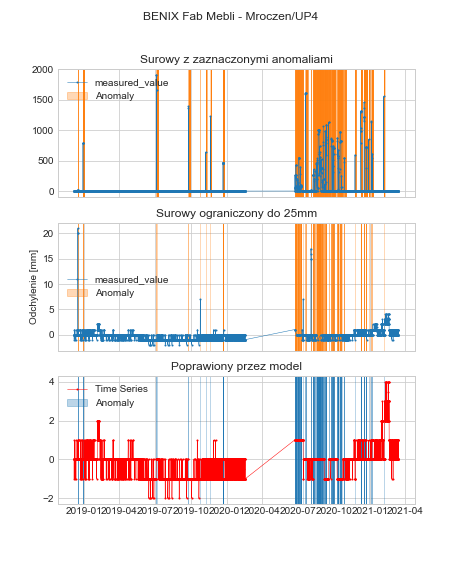
\includegraphics[width=0.9\textwidth]{summary_dev_50.png}

Oczywiste anomalie powyżej 25 mm zostały wykryte i poprawione, a także seria spike'ów od 5 do 25mm.

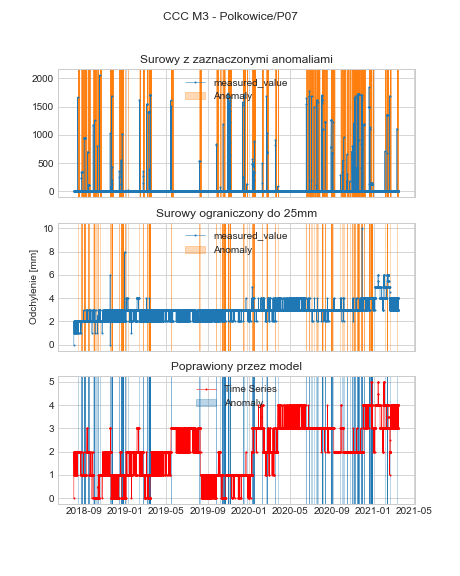
\includegraphics[width=0.9\textwidth]{summary_dev_400.png}

Oczywiste anomalie powyżej 25 mm zostały usunięte, ale także pojedyncze nagłe wzrosty.

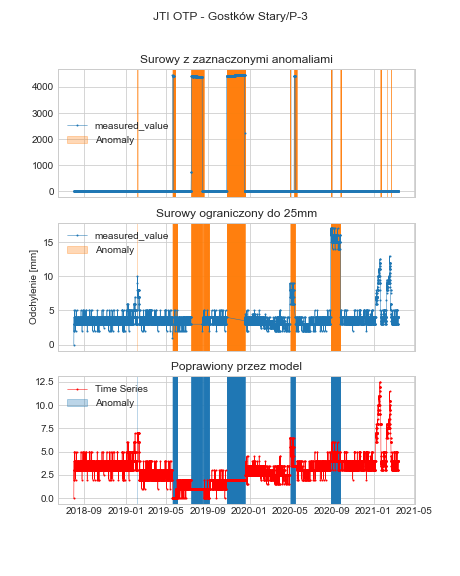
\includegraphics[width=0.9\textwidth]{summary_dev_812.png}

Oczywiste anomalie zostały usunięte, zmiana poziomu została poprawnie skorygowana.

\section{Podsumowanie}
Opracowaliśmy działające rozwiązanie, dysponując narzędziami zgodnymi z aktualnym stanem wiedzy statystycznej. Pozwoliło to uniknąć problemów, z którymi się borykało poprzednie rozwiązanie. Najlepiej widać to na ostatnim rysunku w Sekcji \ref{exampless}.

Stworzony model możemy ulepszyć dokładając do komponentu AR, dodatkowo MA. Wymaga to jednak zapewnienia, że szereg czasowy jest stacjonarny, czego nie możemy być pewni. Zatem najpierw musimy ciąg zróżnicować odpowiednio wiele razy aż stanie się stacjonarny. Taki wariant modelu ARMA nazywa się ARIMA. Szerszy opis tej metody znajduje się w pracy Boxa i Jenkinsa z 2015 roku \cite{arima}.

Utrzymywanie licznika obstrukcji w sposób addytywny jest trudne, ponieważ niesie ryzyko akumulowania addytywnych błędów z czasem. Gdybyśmy jednak chcieli utrzymywać obstrukcję w sposób addytywny, moglibyśmy zaaplikować Filtr Kalmana, używany do korygowania akumulowanych błędów w żyroskopach.
    \printbibliography
    \clearpage
    \appendix
    \section{Przykłady danych}\label{sec:raw-examples}
    \begin{figure}
        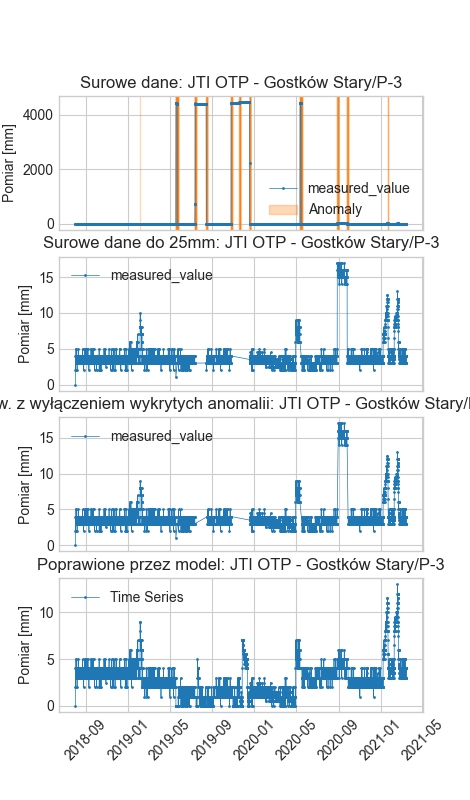
\includegraphics{img_example_812.png}
        \captionof{figure}{Zestawienie wykresów dla JTI OTP - Gostków Stary/P-3.
        \label{fig:example812}}
    \end{figure}
    \begin{figure}
        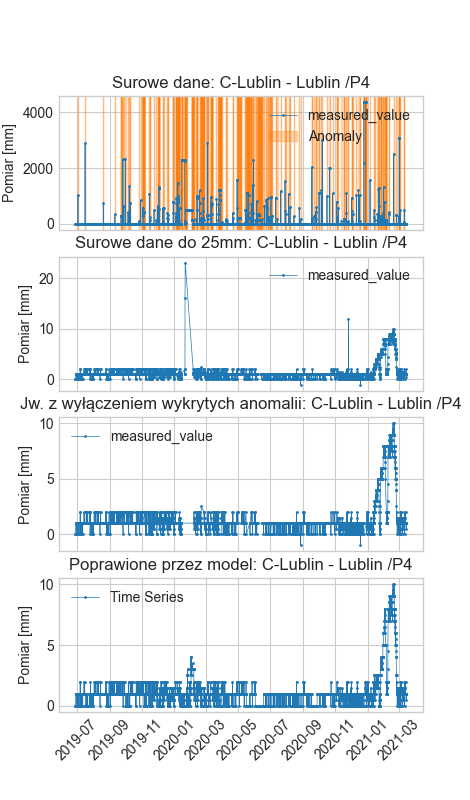
\includegraphics{img_example_201.png}
        \captionof{figure}{Zestawienie wykresów dla C-Lublin - Lublin /P4.
        \label{fig:example201}}
    \end{figure}
    \begin{figure}
        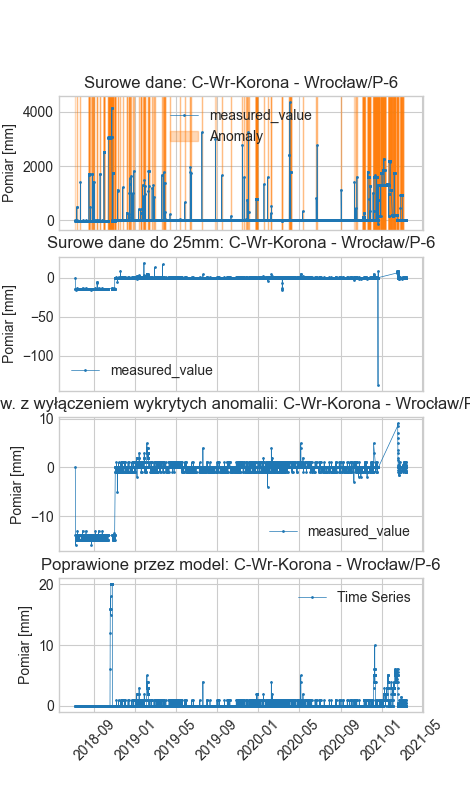
\includegraphics{img_example_305.png}
        \captionof{figure}{Zestawienie wykresów dla C-Wr-Korona - Wrocław/P-6.
        \label{fig:example305}}
    \end{figure}
    \section{Wygenerowane scenariusze}\label{sec:generated-examples}
    \begin{figure}
        \includegraphics{img_example_duży skok.png}
        \captionof{figure}{Scenariusz przedstawia zastawienie na poziomie 1000 mm, które zostaje całkowicie usunięte po pewnym czasie.
        \label{fig:bigjump}}
    \end{figure}
    \begin{figure}
        \includegraphics{img_example_mały skok 7mm.png}
        \captionof{figure}{Scenariusz przedstawia małe zastawienie na poziomie 7 mm, które zostaje całkowicie usunięte po pewnym czasie.
        \label{fig:smalljump7}}
    \end{figure}
    \begin{figure}
        \includegraphics{img_example_mały skok 6mm.png}
        \captionof{figure}{Scenariusz przedstawia małe zastawienie na poziomie 6 mm, które zostaje całkowicie usunięte po pewnym czasie.
        \label{fig:smalljump6}}
    \end{figure}
    \begin{figure}
        \includegraphics{img_example_małe skoki 2mm i spadek.png}
        \captionof{figure}{Scenariusz przedstawia zastawienie rosnące o 2 mm co 3h, które zostaje całkowicie usunięte po pewnym czasie.
        \label{fig:smalljumps2}}
    \end{figure}
    \begin{figure}
        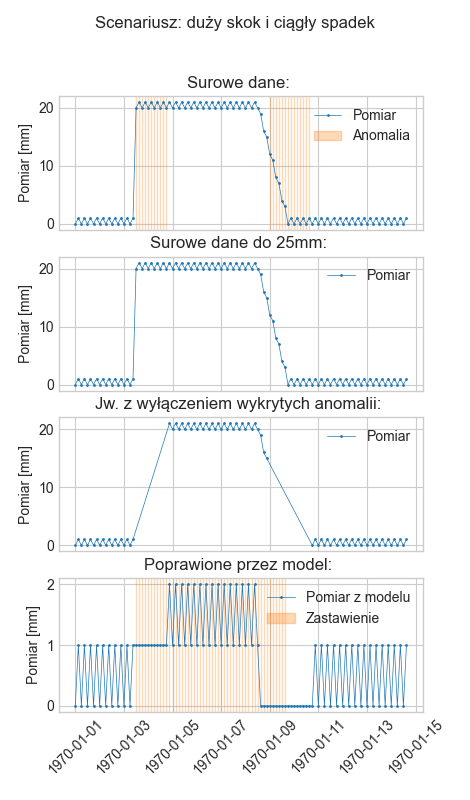
\includegraphics{img_example_duży skok i ciągły spadek.png}
        \captionof{figure}{Scenariusz przedstawia duże zastawienie 20 mm, które zostaje stopniowo usunięte.
        \label{fig:bigjumpcontinous}}
    \end{figure}
    \begin{figure}
        \includegraphics{img_example_duży skok i 3-stopniowy spadek.png}
        \captionof{figure}{Scenariusz przedstawia duże zastawienie 40 mm, które zostaje stopniowo usunięte w trzech krokach.
        \label{fig:bigjump3}}
    \end{figure}
%    {\centering
%    \null\vfill
%    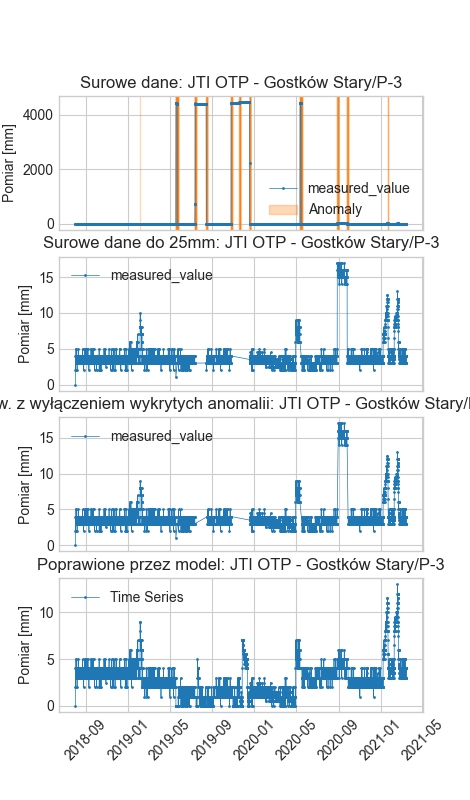
\includegraphics[width=4.5in,201 height=3in]{img_example_812.png}
%    \captionof{figure}{Zestawienie wykresów dla JTI OTP - Gostków Stary/P-3.
%    \label{sec:figmodel1active0yrs}}
%    \vfill
%    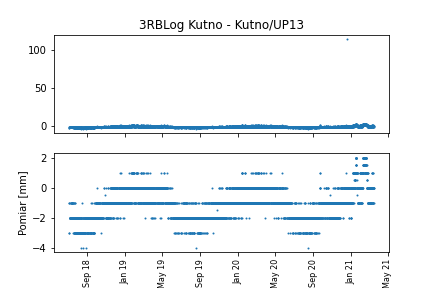
\includegraphics[width=4.5in, height=3in]{example12.png}
%    \captionof{figure}{As-Built Pristine Passive Abutment Fragility Curve%
%    \label{sec:figmodel1passive0yrs}}
%    \vfill\null
%    }
\end{document}
